%! TEX root = ../000-main.tex
\chapter{Non-parametric regression model}
\chaptermark{NP reg. model}

\section{Introduction}

\begin{definition}{Regression function}{}

	Let $(X, Y)$ be random variables with continuous joint distribution.

	The best prediction (in the sense of the minimum mean squared prediction error)
	of the dependent variable $Y$ given that the independent variable $X$ takes
	the known value $x$ is the conditional expectation of $Y$ given $X=x$:
	\begin{equation*}
		m(x) = \mathds{E}( Y \mid X = x)
	\end{equation*}
	also known as \iemph{regression function}.
\end{definition}

\subsection{Parametric regression model}

The \iemph{parametric regression model} assumes that the regression function
is known except for a fixed finite number of parameters.

\begin{example}{Simple linear regression model}{}
	\begin{equation*}
		y = \beta_0 + \beta_1 X + \varepsilon
	\end{equation*}
	So the regression function is $m(x) = \beta_0 + \beta_1 x$ is known except
	for the parameters $\beta_0$ and $\beta_1$.
\end{example}

\subsection{Non-parametric regression model}

In the \iemph{non-parametric regression model} the functional form of the
regression function $m(x)$ is not specified.

\begin{note}
	However, certain regularity conditions are assumed. For instance,
	it is usually assumed that $m(x)$ has a continuous second derivative.
\end{note}

\begin{question}{What does it mean to fit a non-parametric regression model?}{}
	To provide an estimator $\hat{m}(t)$ of the regression function $m(t)$ for
	all $t \in \mathbb{R}$.

	This usually implies to draw the graphic of the pairs $(t, \hat{m}(t))$ where
	$t_j,\, j=1,\ldots,J$ is a regular fine grid covering the range of observed values
	$x_i,\, i=1,\ldots,n$.
	Alternatively, an algorithm that computes the values $\hat{m}(t)$ for any $t$
	can be provided.

	We also have give an estimator $\hat\sigma^2$ of the residual variance $\sigma^2$.
\end{question}

\pagebreak
\section{Local polynomial regression}
\subsection{Local linear regression}

\paragraph{Initial idea} Divide the range of $X$ into $K$ disjoint intervals
each of them showing an \iemph{approximately linear} relationship between $X$ and $Y$.
\begin{figure}[H]
	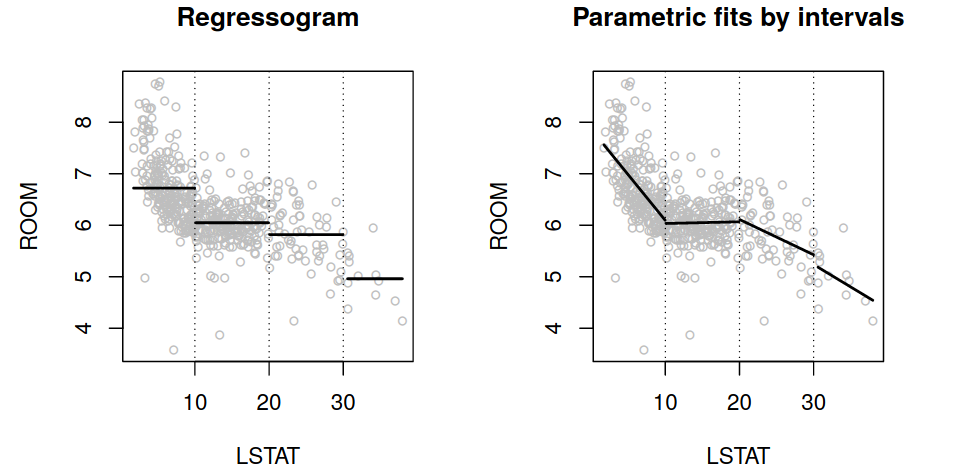
\includegraphics{ll_init}
	\caption{Initial idea of local linear regression.}
\end{figure}

This provides good results, but its not satisfactory, we apply to improvements:
\begin{description}
	\item[Localizing] In order to estimate the regression function at a given value $t$,
		use the data $(x_i, y_i)$ such that $x_i$ is in an interval centered at $t$.
	\item[Smoothing] Assign to each datum $(x_i, y_i)$ a weight $w_i$ that decreases
		as $|x_i - t|$ increases.
\end{description}

\begin{definition}{datum}{}
	A datum is a pair $(x_i, y_i)$ where $x_i$ is the value of the independent
	variable and $y_i$ is the value of the dependent variable.
\end{definition}

\subsubsection{Local linear fitting}
Weights are assigned by a \iemph{kernel function} $K$: usually a
symmetric unimodal density function centered at $0$.

The weight of $(x_i, y_i)$ is when estimating $m(t)$ is:
\begin{equation*}
	w_i = w(t,x_i) = K \left. \left( \frac{x_i - t}{h} \right) \middle/ \sum_{j=1}^n K \left( \frac{x_i - t}{h} \right) \right.
\end{equation*}
where $h$ is the \iemph{smoothing parameter} or \iemph{bandwidth}.

\begin{note}
	The final estimate is significantly affected by the choice of the bandwidth, so this
	choice is crucial in non-parametric estimation.
\end{note}

\begin{figure}[H]
	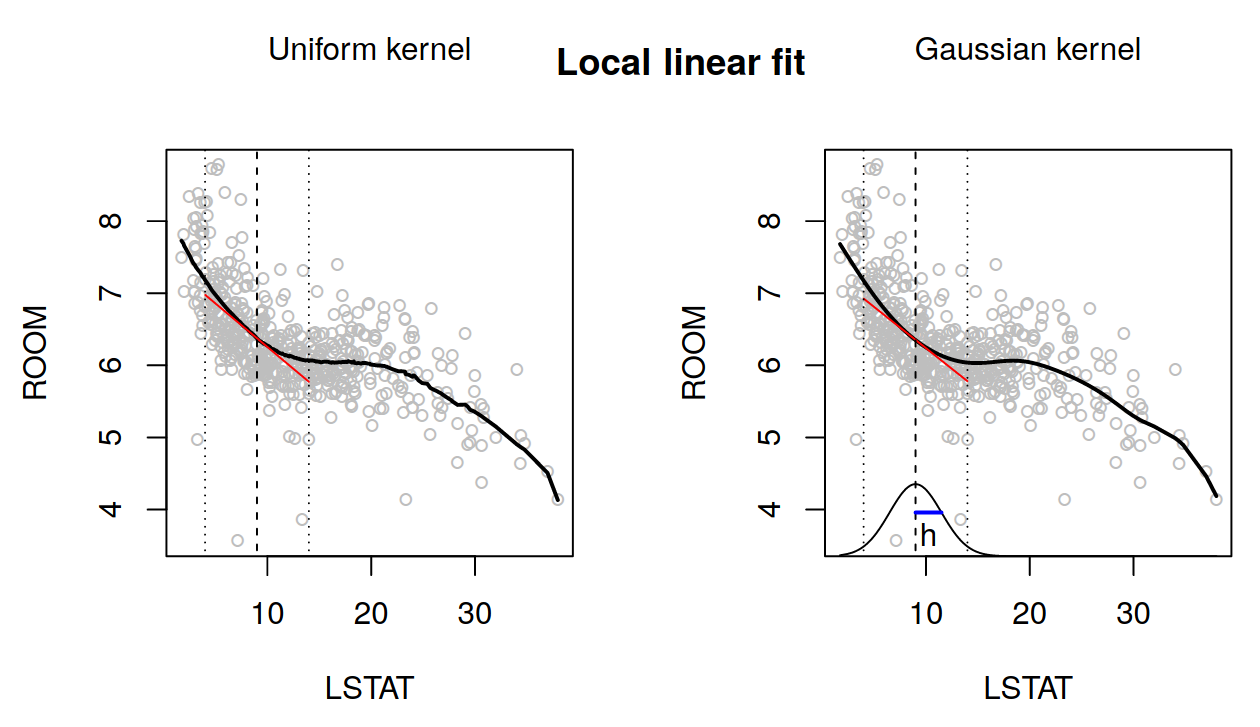
\includegraphics{ll_fit}
	\caption{Local linear fit with different kernel choices.}
\end{figure}

\subsection{Local polynomial regression}
Consider the weighted polynomial regression problem:
\begin{problem}{Weighted polynomial regression problem}{}
\begin{equation*}
	\min_{\beta_0,\ldots,\beta_q} \mathlarger{\sum_{i=1}^n} w_i \left( y_i - \beta_0 - \sum_{j=1}^q \beta_j x_i^j \right)^2
\end{equation*}
\end{problem}
Observe that the estimated coefficients depend on $t$, the
point for which the regression function is being estimated: $\hat\beta_j = \hat\beta_j(t)$.

The proposed estimate for $m(t)$ is the value of the locally fitted
polynomial $P_{q,t}(x) = \sum_{j=0}^q \hat\beta_j(x - t)^j$ at $x = t$:
\begin{equation*}
	\hat{m}(t) = P_{q,t}(t) = \hat\beta_0(t)
\end{equation*}

Moreover, the estimated polynomial $P_{q,t}(x)$ allows us to estimate the first $q$ derivatives
of $m$ at $t$:
\begin{equation*}
	\hat{m}_q^{(r)}(t) = \frac{d^r}{dx^r} P_{q,t}(t) {\Bigm|_{x=t}} = r! \hat\beta_r(t)
\end{equation*}

\subsubsection{Particular case: Nadaraya-Watson estimator}
\begin{definition}{Nadaraya-Watson estimator}{}
	When the degree of the locally fitted polynomial is $q=0$ (i.e. a constant),
	the resulting non-parametric estimator is called \iemph{Nadaraya-Watson estimator}
	or \iemph{kernel estimator}:
	\begin{equation*}
		\hat m_K(t) = \frac{
			\sum_{i=1}^n K \left( \frac{x_i - t}{h} \right) y_i
		}{
			\sum_{i=1}^n K \left( \frac{x_i - t}{h} \right)
		} = \sum_{i=1}^n w(t, x_i) y_i
	\end{equation*}
	\tcblower
	This was proposed before local polynomial estimators.
\end{definition}

Observe that $\hat m_K(t)$ is a moving weighted average.

\begin{prop}{Every local polynomial estimator is itself a weighted average}{}
	\begin{equation*}
		\hat m_{q}(t) = \sum_{i=1}^n w_q^*(t, x_i) y_i
	\end{equation*}
	But the weights $w_q^*(t, x_i)$ are not necessarily non-negative.
\end{prop}

\subsubsection{Matrix formulation of the local polynomial estimator}
Let
\begin{equation*}
	X_t = \begin{pmatrix}
		1      & x_1 - t & \ldots & (x_1 - t)^q \\
		1      & x_2 - t & \ldots & (x_2 - t)^q \\
		\vdots & \vdots  & \ddots & \vdots      \\
		1      & x_n - t & \ldots & (x_n - t)^q
	\end{pmatrix}
\end{equation*}
be the \iemph{regressor matrix}.

We define $Y = (y_1, \ldots, y_n)^T,\, \varepsilon = (\varepsilon_1, \ldots, \varepsilon_n)^T,\,
	\beta = (\beta_0, \ldots, \beta_q)^T$ and we let $W_t = \text{diag}(w(x_1, t), \ldots, w(x_n,t))$
be the \iemph{weight matrix}.

We fit the regression model $Y = X_t\beta + \varepsilon$ using weighted least squares:
\begin{align*}
	\hat\beta & = \argmin_{\beta\in\mathbb{R}^{q+1}} \sum_{i=1}^n w_i(y_i - \beta_0 - \sum_{j=1}^q \beta_j x_i^j)^2 \\
	          & = \argmin_{\beta\in\mathbb{R}^{q+1}} (Y - X_t\beta)^T W_t (Y - X_t\beta)
\end{align*}
The solution is:
\begin{equation*}
	\hat\beta = (X_t^T W_t X_t)^{-1} X_t^T W_t Y
\end{equation*}

For $j=0,\ldots,q$, let $e_j$ be the $(q+1)$-dimensional vector
having all its coordinates 0 except for the $(j+1)$-th one, which is 1.
Then:
\begin{equation*}
	\hat m_q(t) = \hat \beta_0 = e_0^T (X_t^T W_t X_t)^{-1} X_t^T W_t Y = S_tY = \sum_{i=1}^n w^*_q(t, x_i) y_i
\end{equation*}
where $S_t = e_0^T (X_t^T W_t X_t)^{-1} X_t^T W_t$ is an $n$-dimensional row vector (it
is in fact a \iemph{smoothing matrix}).

\begin{note}
	We say that the local polynomial regression estimator is a \iemph{linear smoother}
	because for a fixed $t$, $\hat m_q(t)$ is a linear function of $y_1,\ldots,y_n$.
\end{note}

The local polynomial estimator of the $r$-th derivative of $m$ at point $t$ is:
\begin{equation*}
	\hat m_q^{(r)}(t) = r!e_r^T\hat\beta_r(t) = r!e_r^T\hat\beta
\end{equation*}
which is also linear in $y_1,\ldots,y_n$.

\subsection{Linear smoothers}

\begin{definition}{Linear smoother}{}
	A non-parametric linear regression estimator $\hat m$ is said to be
	a \iemph{linear smoother} when for any fixed $t$, $\hat m(t)$ is a linear function of
	$y_1,\ldots,y_n$:
	\begin{equation*}
		\hat m(t) = \sum_{i=1}^n w(t, x_i) y_i
	\end{equation*}
	for some weight function $w$.
	\tcblower
	\begin{note}
		Linear smoothers are particular cases of linear estimators of the regression
		function, as \iemph{OLS} or \iemph{ridge regression}.
	\end{note}
\end{definition}

\begin{definition}{Smoothing matrix}{}

	Let
	\begin{equation*}
		\hat y_i = \hat m (x_i) = \sum_{j=1}^n w(x_i, x_j) y_j
	\end{equation*}
	be the fitted values for the $n$ observed values  $x_i$ of the explanatory variable.

	In matrix format:
	\begin{equation*}
		\hat Y = S Y
	\end{equation*}
	where column vectors $Y$ and $\hat Y$ have elements $y_i$ and $\hat y_i$ respectively,
	and the matrix $S$ has generic element $s_{ij} = w(x_i, x_j)$.

	\begin{note}
		The matrix $S$ is called the \iemph{smoothing matrix}, because its effect on the observed
		data $(x_i, y_i)$ is to transform them into $(x_i, \hat y_i)$ which is a much
		smoother data configuration.
	\end{note}

	\tcblower
	The smoothing matrix is analogous to the \iemph{hat matrix} $H = X(X^TX)^{-1}X^T$ in
	multiple linear regression:
	\begin{equation*}
		\hat Y = X(X^TX)^{-1}X^T Y = H Y
	\end{equation*}
\end{definition}

\begin{prop}{Parameters in a linear smoother model}{}
	For a linear smoother with smoothing matrix $S$, the \iemph{effective
		number of parameters} is the sum of diagonal elements of $S$:
	\begin{equation*}
		\nu = \text{Trace}(S) = \sum_{i=1}^n s_{ii}
	\end{equation*}
	\tcblower
	\begin{note}
		The interpretation of $\nu$ as the effective number of parameters is
		valid for any linear non-parametric estimator.
	\end{note}

	We can thus compare the degree of smoothing of two linear non-parametric
	estimators just by comparing their effective number of parameters.
\end{prop}

\subsubsection{An estimator of $\sigma^2$}
An estimator of $\sigma^2$ in non-parametric estimation is:
\begin{equation*}
	\hat\sigma^2 = \frac{1}{n-\nu} \sum_{i=1}^n (y_i - \hat m(x_i))^2
\end{equation*}

\subsection{Kernel functions}

\begin{definition}{Kernel functions}{}
    Density functions with zero mean.
    \tcblower
    We can also rescale them so that they have zero mean and
    variance 1. Then we call them \iemph{rescaled kernels}.
\end{definition}

\begin{figure}[H]
	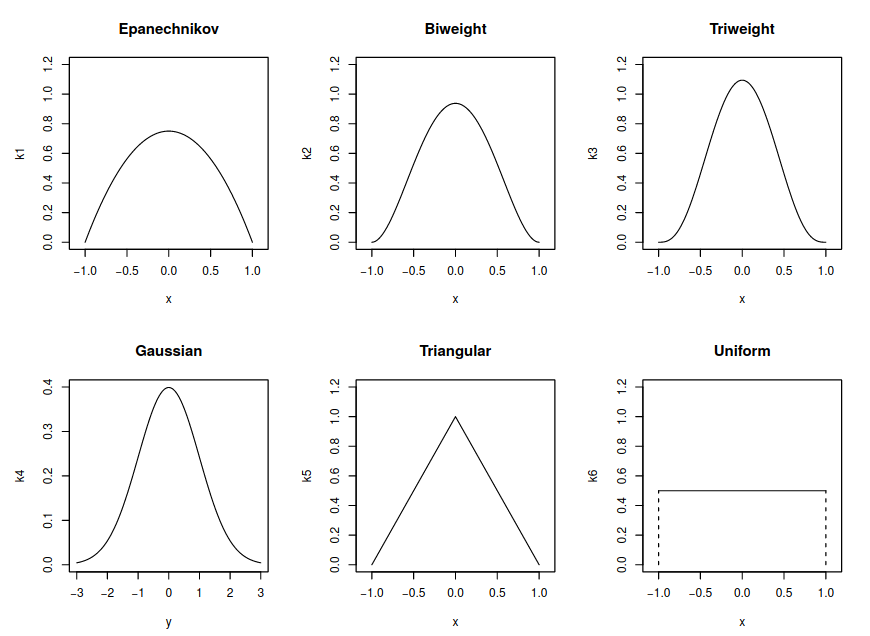
\includegraphics{kernel_examples}
	\caption{Examples of Kernel functions used in non-parametric estimation}
\end{figure}

\begin{table}[H]
	\begin{tabular}{lccl}
		\toprule
		Kernel ($K$)         & Expression                                & Variance & Efficiency \\
		\midrule
		Epanechnikov ($K^*$) & $\frac{3}{4}(1-x^2)I_{[-1,1]}(x)$         & $1/5$    & 1          \\
		Biweight             & $\frac{15}{16}(1-x^2)^2I_{[-1,1]}(x)$     & $1/7$    & 0.994      \\
		Triweight            & $\frac{35}{32}(1-x^2)^3I_{[-1,1]}(x)$     & $1/9$    & 0.987      \\
		Gaussian             & $\frac{1}{\sqrt{2\pi}}e^{-\frac{x^2}{2}}$ & $1$      & 0.951      \\
		Triangular           & $\frac{1}{2}(1-|x|)I_{[-1,1]}(x)$         & $1/6$    & 0.986      \\
		Uniform              & $\frac{1}{2}I_{[-1,1]}(x)$                & $1/3$    & 0.930      \\
		\bottomrule
	\end{tabular}
\end{table}

\section{Linear smoothers}
\section{Choosing the smoothing parameter}
